\section{Experiments and Results}\hfill

\textbf{\myname{} Setup:} We deploy \myname{} with each encoder block stacked three times to achieve a deeper representation of jets. We schedule the learning rate to decay by a factor of 0.1 after the $25^{th}$ epoch which noticeably helped descend the noisy loss landscape in model training. The \emph{AdamW} optimizer is used to prevent overtraining using weight decay and we use $R^2$ as an evaluation metric. The model converged after training 50 epochs on an NVIDIA RTX 3090.\\

\begin{figure}[ht!]
\begin{subfigure}{.25\textwidth}
  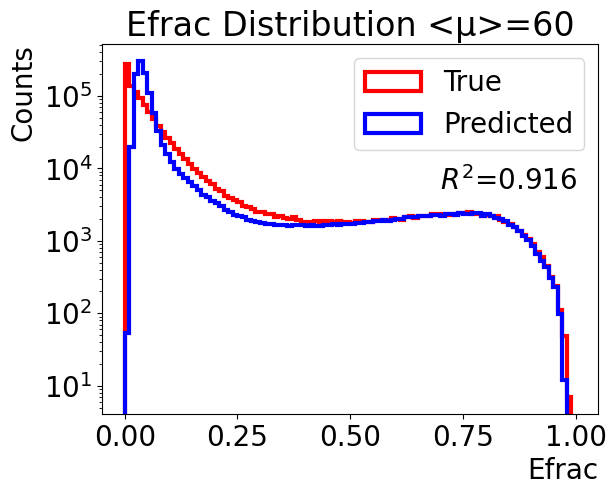
\includegraphics[width=1\linewidth]{Efrac1D_mu60.png}
  \caption{}
  \label{fig:Efrac1d_mu60}
\end{subfigure}%
\begin{subfigure}{.25\textwidth}
  \includegraphics[width=1\linewidth]{Efrac2d_mu60.png}
  \caption{}
  \label{fig:Efrac2d_mu60}
\end{subfigure}
\begin{subfigure}{.25\textwidth}
  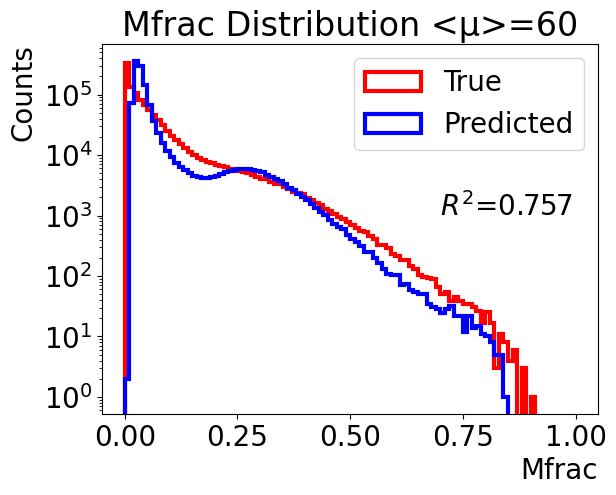
\includegraphics[width=1\linewidth]{Mfrac1D_mu60.png}
  \caption{}
  \label{fig:Mfrac1d_mu60}
\end{subfigure}%
\begin{subfigure}{.25\textwidth}
  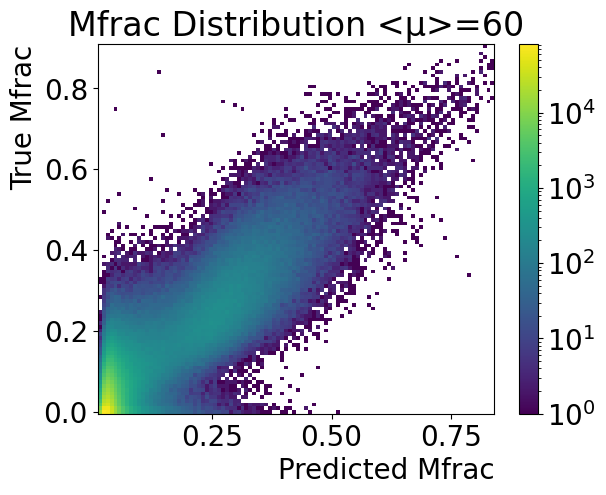
\includegraphics[width=1\linewidth]{Mfrac2D_mu60.png}
  \caption{}
  \label{fig:Mfrac2d_mu60}
\end{subfigure}
\begin{subfigure}{.25\textwidth}
  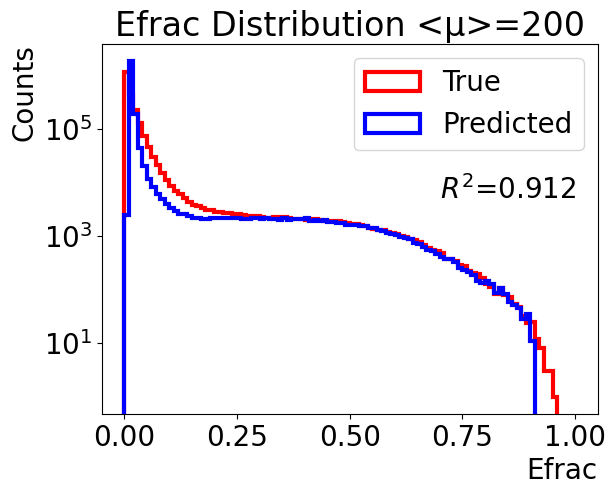
\includegraphics[width=1\linewidth]{Efrac1D_mu200.png}
  \caption{}
  \label{fig:Efrac1d_mu200}
\end{subfigure}%
\begin{subfigure}{.25\textwidth}
  \includegraphics[width=1\linewidth]{Efrac2d_mu200.png}
  \caption{}
  \label{fig:Efrac2d_mu200}
\end{subfigure}
\begin{subfigure}{.25\textwidth}
  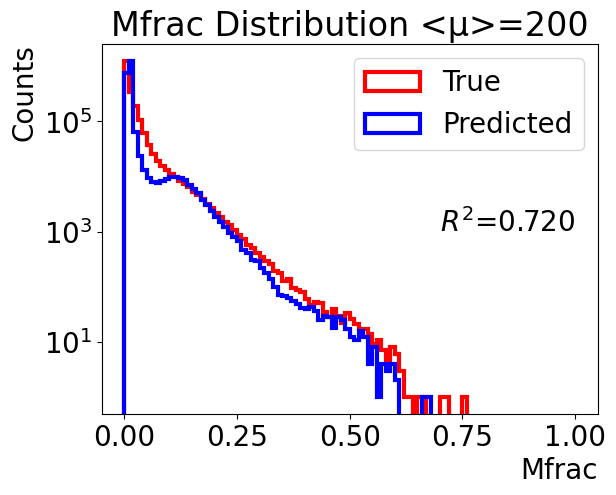
\includegraphics[width=1\linewidth]{Mfrac1D_mu200.png}
  \caption{}
  \label{fig:Mfrac1d_mu200}
\end{subfigure}%
\begin{subfigure}{.25\textwidth}
  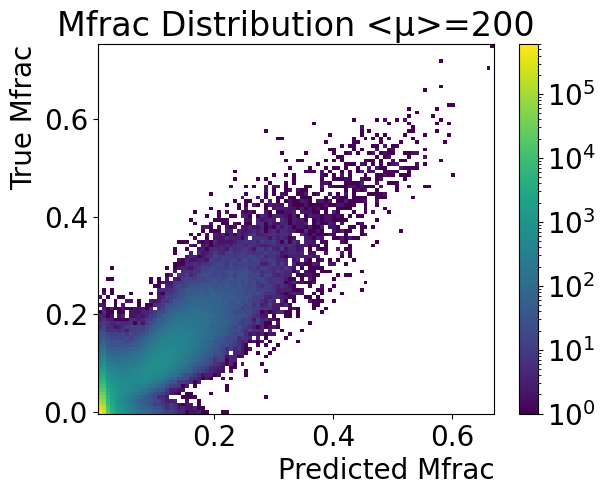
\includegraphics[width=1\linewidth]{Mfrac2D_mu200.png}
  \caption{}
  \label{fig:Mfrac2d_mu200}
\end{subfigure}
\caption{At $\left \langle \mu \right \rangle=60$ (top row) and $\left \langle \mu \right \rangle=200$ (bottom row), the predicted energy (left) and mass (right) fraction of jets shown as 1D and 2D histograms.}
\label{fig:RegressionResults}
\end{figure}

\textbf{Regression Results:} \myname{} was evaluated on a sample of 20k di-Higgs events simulated specifically for testing. At $\left \langle \mu \right \rangle=60$, the model achieves $R^2=0.916$ for $E_{frac}$, as shown in Figure~\ref{fig:Efrac1d_mu60}, and $R^2=0.757$ for $M_{frac}$, as shown in Figure~\ref{fig:Mfrac1d_mu60}. At $\left \langle \mu \right \rangle=200$, the model achieves $R^2=0.912$ for $E_{frac}$, as shown in Figure \ref{fig:Efrac1d_mu200}, and $R^2=0.720$ for $M_{frac}$, as shown in Figure \ref{fig:Mfrac1d_mu200}. The 2D predicted vs truth values, plotted with a log z color scale, shown in Figure [\ref{fig:Efrac2d_mu60},\ref{fig:Mfrac2d_mu60}] at $\left \langle \mu \right \rangle=60$ and in Figure \ref{fig:Efrac2d_mu200} \ref{fig:Mfrac2d_mu200} at $\left \langle \mu \right \rangle=200$, show that there is good diagonal trend between the predictions and the truth. Overall, the transformer encoder architecture provides a highly parallelizable algorithm that is computationally feasible at high pileup conditions, and the plots in Figure~\ref{fig:RegressionResults} show that \myname{} learns the hard scatter contributions without significant degradation to the $R^2$ value at high pileup conditions of the HL-LHC.

%\luke{Move part of this discussion to the Jet Labels section}It is clear from the 2D histograms that the model performs noticeably better on Efrac than Mfrac, which is expected due to the physics. Energy fraction is analogous to a scalar sum while mass fraction is analogous to vector sum. Pileup contamination typically has low energy and therefore does not affect the scalar sum as much as the stochastic direction vectors affect the vectorial sum used to calculate mass fraction. The model is very good at identifying hard scatter jets, with energy fraction close to one, but the model does not perform as well with pileup jets, energy fraction close zero. However, its important to note that the hard scatter jets are of most interest to physics, and there is very good energy fraction modeling in this region. \\

\newpage
\textbf{Classic JVT Benchmark:} In order to benchmark the performance of the model against existing JVT algorithm, only a subset of the model is used to maintain consistency across input features. For a fair comparison, only jet features are considered: \{$p_T,\eta,\phi,m,R_{p_T},corrJVF$\} where $R_{p_T}$ and $corrJVT$ are defined in ~\cite{ATLAS-CONF-2014-018}. This exercise attempts to show that the attention architecture over jet features (AttnJVT) alone brings noticeable improvements when jets are processed in the context of an event. These results can be further improved when jets are compounded with track features.

\begin{figure}[ht]
\centering
\begin{subfigure}{.32\textwidth}
  \centering
  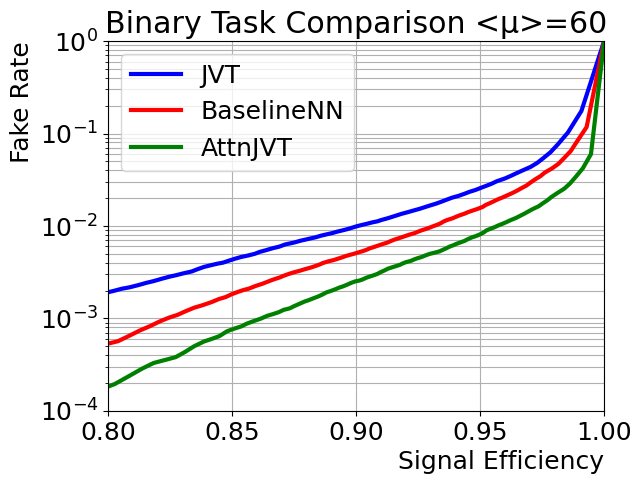
\includegraphics[width=1\linewidth]{JVT_Benchmark_mu60.png}
  \caption{}
  \label{fig:Benchmark:sub1}
\end{subfigure}%
\begin{subfigure}{.32\textwidth}
  \centering
  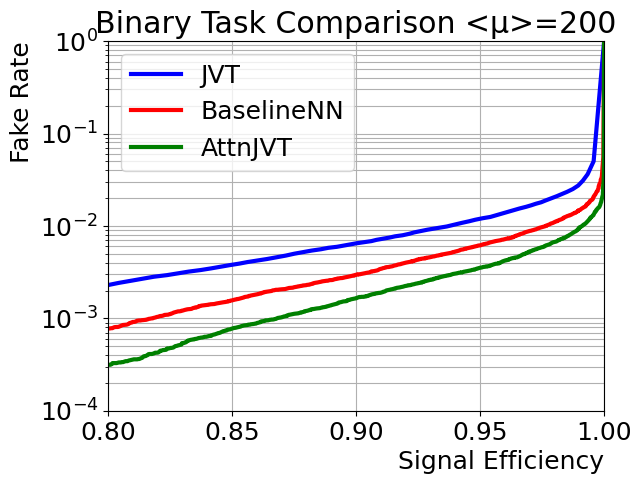
\includegraphics[width=1\linewidth]{JVT_Benchmark_mu200.png}
  \caption{}
  \label{fig:Benchmark:sub2}
\end{subfigure}
\begin{subfigure}{.32\textwidth}
  \centering
  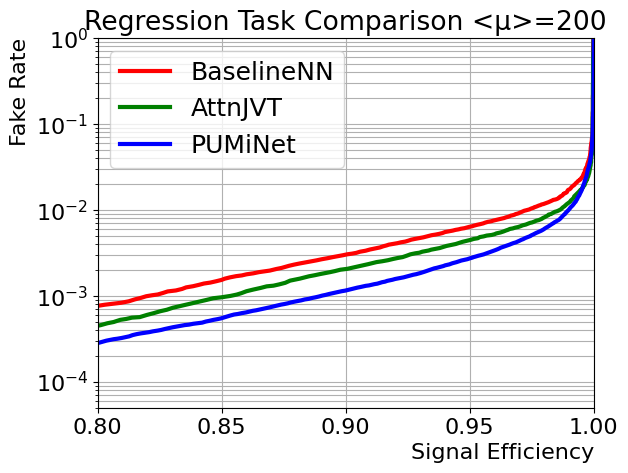
\includegraphics[width=1\linewidth]{ROC_Comparison_wtracks.png}
  \caption{}
  \label{fig:Benchmark:sub3}
\end{subfigure}
\caption{Benchmark performance for the binary classification task for replica ATLAS JVT (blue), baseline deep NN (red), and MHA jet encoder (green) for for $\left<\mu\right>=60$ (a) and $\left<\mu\right>=200$ (b). Further improvement can be gained by \myname{} when tracks are added to the model (c). }
\label{fig:Benchmark}
\end{figure}

Using the di-Higgs dataset, the following models were created: (1) a replica of ATLAS JVT kNN model described in ~\cite{ATLAS-CONF-2014-018} (2) a baseline deep neural network, and (3) a single MHA encoder between jets, AttnJVT.\footnote{A small number of learnable parameters are used, 21k, for AttnJVT and the baseline deep NN.} Since JVT is a binary classifier, the continuous labels are converted to binary using a cut at $E_{frac}=0.3$. The JVT algorithm and deep NN process inputs on a per jet basis, but AttnJVT processes an entire set of jets in the context of an event which allows the model to capture correlations between hard scatter jets. The baseline deep NN and AttnJVT are trained using the Binary Cross Entropy loss function, and converges after 60 epochs on 50k events. The benchmarked false positive rates against the true positive rates are shown in Figure Figure \ref{fig:Benchmark:sub1} \& \ref{fig:Benchmark:sub2} which shows that AttnJVT can significantly lower the false positive rate. We also show that \myname{} brings further improvements over AttnJVT using both jet and track features to capture event-wide correlations in the regression setup, as shown in Figure \ref{fig:Benchmark:sub3}.
